\chapter{Техника эксперимента} \label{chapt_exp_tech}
\section{Дифракция медленных электронов} \label{leed}
Дифракция медленных электронов (ДМЭ) позволяет исследовать структуру поверхностных слоев кристаллов.  В настоящей работе ДМЭ использовалась для определения взаимного расположения графена и подложки, а также для контроля качества исследуемой системы. На Рис. \ref{img:leed_scheme} показана экспериментальная реализация данного метода. Основные части установки - это электронная пушка, набор металлических сеток, держатель образца и флюоресцентный экран. В ходе измерения образец помещается в центр полусферы, электроны эмитируются катодом электронной пушки, разгоняются до необходимой энергии (20-200 эВ), движутся в бесполевом пространстве по направлению к образцу и рассеиваются на его приповерхностных слоях. Тормозящие сетки отсекают неупруго рассеянные электроны. Пучки упруго рассеянных электронов, прошедшие сетки, ускоряются до энергий 5-7 кэВ и попадают на флюоресцентный экран, после чего на нем наблюдают дифракционную картину. 
Для исследования атомной структуры приповерхностных слоев энергия первичных электронов должна удовлетворять условию наблюдения дифракционной картины: длина волны электрона $\lambda$ должна быть сравнима с расстояниями между атомами. Длина волны де-Бройля для электронов определяется из соотношений
 	\begin{equation}
  \label{eq:equation1}
 \lambda=\frac{h}{p}=\frac{h}{\sqrt{2mE}}, \lambda[\buildrel _\circ \over {\mathrm{A}}]\approx\frac{150}{E[eV]}.
\end{equation}
Высокая поверхностная чувствительность метода ДМЭ определяется тем, что при таких энергиях длина свободного пробега электрона составляет несколько атомных слоев, и поэтому большинство актов упругого рассеяния происходит в верхних слоях кристалла.
 \begin{figure}[ht] 
  \center
  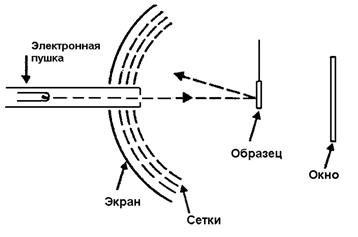
\includegraphics [scale=1] {./Dissertation/images/leed_scheme.jpg}
  \caption{Схема стандартного эксперимента по ДМЭ.} 
  \label{img:leed_scheme}  
\end{figure}
 

Пусть $\overrightarrow{k}$ и $\overrightarrow{k'}$ — волновые векторы падающей и рассеянной электронной волны. Представим их в виде суммы двух компонент, одна из которых параллельна плоскости поверхности, а другая ей перпендикулярна: $\overrightarrow{k}=\overrightarrow{k_\perp}+\overrightarrow{k_\parallel}$ (аналогично для $\overrightarrow{k'}$). Для квазидвумерных систем, когда периодичность структуры наблюдается только в плоскости параллельной поверхности, при рассеянии электронной волны сохраняется лишь компонента волнового вектора $k_\parallel$ (с добавлением вектора обратной решётки $\overrightarrow{g_{h_k}}$.На основании законов сохранения энергии и импульса справедливы следующие соотношения:
 	\begin{equation}
  \label{eq:equation100}
\overrightarrow{k}=\overrightarrow{k'}
\end{equation}
или
 	\begin{equation}
  \label{eq:equation1}
\overrightarrow{k_\parallel}+\overrightarrow{k_\perp}=\overrightarrow{k'_\parallel}+\overrightarrow{k'_\perp}
\end{equation}
 	\begin{equation}
  \label{eq:bragg}
\overrightarrow{k'_\parallel}=\overrightarrow{k_\parallel}+\overrightarrow{g_{h_k}},  \overrightarrow{g_{h_k}}=h\overrightarrow{a^*}+k\overrightarrow{b^*}.
\end{equation}


Базисные векторы трансляции обратной решётки $\overrightarrow{a^*}$и $\overrightarrow{b^*}$ связаны с векторами решётки в прямом пространстве $\overrightarrow{a}$ и $\overrightarrow{b}$ соотношениями

 	\begin{equation}
  \label{eq:equation1}
\overrightarrow{a^*}=\frac{\overrightarrow{b}\times\overrightarrow{n}}{A},  \overrightarrow{b^*}=\frac{\overrightarrow{n}\times\overrightarrow{a}}{A},  A=\overrightarrow{a}\cdot\overrightarrow{b}\times\overrightarrow{n}.
\end{equation}

где $\overrightarrow{n}$ — единичный вектор нормали к поверхности.
Выражения (\ref{eq:equation100}–\ref{eq:bragg}), представляют собой закон Брэгга,
описывающий условия конструктивной интерференции падающей и рассеянной волны. Таким образом, дифрагированным пучкам соответствуют индексы обратной решётки ($hk$) (в трёхмерном случае — $hkl$). По их расположению можно сделать вывод о симметрии обратной решётки, а значит, используя уравнения (\ref{eq:bragg}), и о структуре решётки в прямом пространстве.
\section{Фотоэлектронная спектроскопия остовных уровней}
Фотоэлектронная спектроскопия (ФЭС) является мощным инструментом для исследования поверхности твердых тел.

В данном методе исследуемый образец подвергается воздействию рентгеновского или ультрафиолетового излучения. Затем спектр фотовозбужденных электронов регистрируется с высоким энергетическим разрешением. Существует две разновидности ФЭС. В одном варианте регистрируются и анализируются спектры фотоэлектронов, эмитированных при возбуждении остовных уровней, в другом исследуются спектры электронов валентной зоны. В первом случае спектр является дискретным, причем каждая его линия характеризует возбуждение фотоэлектронов с определенных атомных уровней. Энергии связи остовных электронов специфичны для разных элементов, следовательно, можно установить, из каких элементов состоит приповерхностная область образца. Кроме того, величина энергии связи зависит от химического окружения атома, и поэтому измерение положения остовных уровней используется для определения химических соединений. Анализ таких энергетических сдвигов стал возможным благодаря появлению мощных источников синхротронного излучения. Они значительно расширили возможности метода спектроскопии остовных уровней, превратив его в эффективный метод исследования поверхности твердого тела. 

Рассмотрим физические основы метода. Диаграмма, иллюстрирующая процесс фотоэмиссии остовного электрона, показана в левой части Рис. \ref{img:pes}. Энергия связи $E_i$ остовного электрона в твердом теле отсчитывается относительно уровня Ферми, а не относительно уровня вакуума как в свободном атоме. Поэтому кинетическая энергия электрона ($E$), возбужденного с $i$-го уровня фотоном с энергией $h\nu$, равна: 
 	\begin{equation}
  \label{eq:equation101}
E=h\nu-E_i -e\phi,
\end{equation}
где $e\phi$ – это работа выхода материала, а величина $Е$ рассчитывается относительно уровня вакуума.

Из этой формулы видно, что энергия связи $E_i$ остовного фотоэлектрона определяется только его кинетической энергией при заданной величине $h\nu$ и известном значении $e\phi$. В экспериментальных условиях, кроме того, возникает контактная разность потенциалов $U_c$ между эмиттером и спектрометром, которая влияет на энергию возбужденных электронов, и изменяет ее значение на величину $еU_c$. Данная величина определяется как разница между работой выхода материала образца и работой выхода материала спектрометра ($U_s$). Принимая во внимание данный фактор, из формулы \ref{eq:equation101} получается следующее выражение для расчета энергии связи остовного фотоэлектрона:
 	\begin{equation}
  \label{eq:equation102}
E=h\nu-E_{kin} -e\phi_s,
\end{equation}
где $E_{kin}$ – измеряемое значение кинетической энергии фотоэлектрона (см. \ref{img:pes}).

 \begin{figure}[ht] 
  \center
  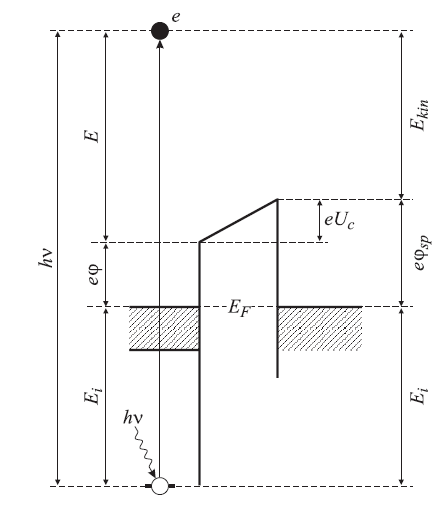
\includegraphics [scale=0.47] {./Dissertation/images/pes.png}
  \caption{Схематическая диаграмма, иллюстрирующая процесс возбуждения остовного электрона.} 
  \label{img:pes}  
\end{figure}


Таким образом, для того, чтобы определить энергию связи фотоэлектрона, нет необходимости знать работу выхода исследуемого образца. Требуется только рассчитать значение $e\phi_s$, которое находят при калибровке спектрометра с использованием эталонного образца. Легко видеть, что в случае металла энергия связи остовного электрона может быть также определена из сопоставления его кинетической энергии и кинетической энергии возбужденного с уровня Ферми металла валентного электрона. 
В рамках представленной на Рис. \ref{img:pes} модели, предполагается, что электроны, выходя из образца, не испытывают неупругих потерь энергии. Это происходит, если фотоэлектроны возбуждаются в относительно тонком приповерхностном слое толщиной меньшей, чем средняя длина свободного пробега ($\lambda$) до момента неупругого рассеяния. Величина длины свободного пробега зависит от энергии электрона, а эта зависимость имеет сходный вид для всех материалов (Рис. \ref{img:pes2}) с минимумом в области энергий порядка нескольких десятков эВ.
 \begin{figure}[ht] 
  \center
  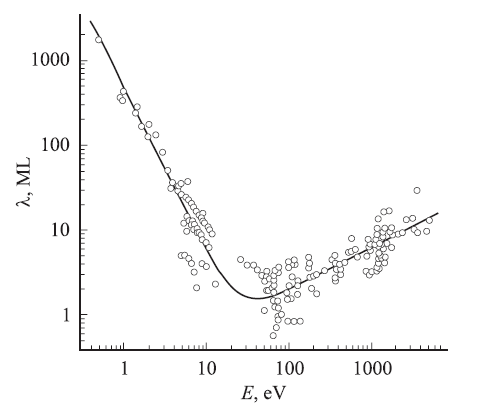
\includegraphics [scale=0.67] {./Dissertation/images/pes2.png}
  \caption{Зависимость средней длины свободного пробега электрона от энергии.} 
  \label{img:pes2}  
\end{figure}
 

Если глубина выхода фотоэлектрона без потерь энергии значительно превышает толщину приповерхностного слоя, то главный вклад в линию спектра вносят фотоэлектроны, эмитируемые атомами из объема, а спектр при этом называется объемно-чувствительным. Если же эти параметры имеют сопоставимые величины, то электроны, испускаемые атомами приповерхностной области, вносят значительный вклад в линию спектра, и такой спектр является поверхностно-чувствительным. Ясно, что для того, чтобы спектр был наиболее чувствительным к состоянию поверхности, энергии фотоэлектронов должны соответствовать минимуму зависимости $\lambda$(Е). Как правило, этого можно достигнуть выбором энергии фотонов. Объемно-чувствительный спектр принято измерять при энергиях, которые находятся на ниспадающей части зависимости $\lambda$(Е), где величина $\lambda$ сильно понижается при увеличении энергии. В таком случае для того, чтобы перейти от объемно-чувствительного спектра к поверхностно-чувствительному, достаточно понизить энергию фотонов лишь на несколько десятков электрон-вольт. Чтобы дополнительно усилить вклад приповерхностной области в спектре, необходимо увеличить полярный угол вылета исследуемых фотоэлектронов. Чем больше значение этого угла (отсчитываемое от нормали к поверхности), тем меньше глубина выхода электронов, и тем более значительный вклад в общий спектр дают поверхностные атомы. 
Как уже было отмечено, для практической реализации метода требуется применение синхротронного источника излучения, который имеет высокую плотность потока фотонов, а также дает возможность изменять их энергию. Кроме того, требуется наличие электронного спектрометра, обладающего достаточно высоким энергетическим разрешением.
Необходимо также отметить, что спектры остовных уровней обычно приводят в виде зависимости интенсивности фотоэлектронов от энергии связи. При этом за ноль шкалы энергий принимают либо энергию на уровне Ферми изучаемого образца, либо энергию связи электронов из атомов объема. Во втором случае атомы поверхности, остовные уровни которых имеют бóльшую энергию связи, чем атомы объема, имеют положительный энергетический сдвиг. Как правило, при этом приводят лишь узкий участок спектра вблизи выбранной линии.

\section{ Фотоэлектронная спектроскопия с угловым разрешением}  \label{chapt3}
ФЭСУР является основным методом для получения дисперсионных зависимостей $E(\overrightarrow{k})$ электронных состояний валентной зоны кристаллов. Для исследований зонной структуры методом ФЭСУР обычно выбирают такие энергии фотонов, при которых происходит прямой переход электрона в возбуждённое состояние, т.е. изменение энергии фотоэлектрона происходит при сохранении его импульса. Иными словами, импульс фотона должен быть пренебрежимо мал по сравнению с размерами зоны Бриллюэна кристалла. С другой стороны, энергию фотонов не следует выбирать слишком маленькой, чтобы конечное состояние возбуждённого электрона описывалось уже не блоховской волновой функцией, а плоской волной с параболическим законом дисперсии, иначе вместо плотности начальных состояний придётся иметь дело с приведённой плотностью начальных и конечных состояний.
При фотовозбуждении происходит прямой переход электрона из состояния в валентной зоне с квазиимпульсом $k_i$, описываемого блоховской функцией, в состояние плоской волны с импульсом $k_f$, при этом $k_f=k_i$.  Удобно разложить векторы импульса фотоэлектрона до (индекс $in$) и после ($out$) выхода из кристалла в вакуум на составляющие, параллельные ($\parallel$) и перпендикулярные ($\perp$) плоскости поверхности:
 	\begin{equation}
  \label{eq:arpes2}
k_f=k^{in}_\parallel+k^{in}_\perp, k^{out}=k^{out}_\parallel+k^{out}_\perp
\end{equation}

Поскольку при переходе через поверхность электрон теряет часть своей энергии (на величину работы выхода), перпендикулярная составляющая им
пульса $k^{in}_\perp$ уменьшается, при этом параллельная компонента $k^{in}_\parallel$ сохраняется с точностью до вектора обратной решётки кристалла $G$: $k^{out}_\parallel=k^{in}_\parallel+G$. Если рассматривать только первую зону Бриллюэна, т.е. работать в приведённой зонной схеме, можно считать $k^{out}_\parallel=k^{in}_\parallel$ . При выходе электрона в вакуум происходит изменение направления его движения. Зная угол $\theta$ и измеряя кинетическую энергию движущегося в вакууме в данном направлении фотоэлектрона, можно получить следующее выражение для $k^{in}_\parallel$:
\begin{equation}
\label{eq:arpes}
k^{in}_\parallel=k^{out}_\parallel sin\theta=\sqrt{\frac{2m}{h^2}E_{kin}}sin\theta
\end{equation}
Выражение \ref{eq:arpes} является основным в методе ФЭСУР. Меняя полярный угол $\theta$ и измеряя ФЭ спектр, можно получить набор данных $E^{in}_B(k_\parallel)$, т.е. дисперсионную зависимость в спроецированной на поверхность зоне Бриллюэна вдоль направления, задаваемого азимутальным углом $\phi$. Для двумерных систем, таких как графен, этого достаточно для построения полной картины дисперсии зон, потому что зона Бриллюэна двумерна. В случае же трёхмерных систем ситуация более сложная, так как для определения зависимости $E^{in}_B(k_\perp)$ необходимо получить спектры при разных энергиях фотонов.
 Пучок фотонов, попадая на образец, вызывает эмиссию первичных и вторичных электронов, распределение по энергии и углам которых регистрируется с помощью полусферического анализатора. Поскольку данный метод требует измерений зависимости энергетического спектра фотоэлектронов от направления их движения $\theta$, высокое угловое разрешение анализатора является одним из самых важных условий.

\section{ Ближняя тонкая структура рентгеновских спектров поглощения}
Спектроскопия поглощения рентгеновского излучения основана на измерении зависимости коэффициента поглощения излучения от энергии фотонов. Примерный вид такой зависимости приведён на Рис. \ref{img:nexafs}. Её характерными особенностями являются: (i) наличие резких скачков в коэффициенте поглощения при определённых энергиях, называемых краями поглощения; (ii) за этими краями наблюдается убывание коэффициента поглощения; (iii) чуть выше краёв видна так называемая тонкая структура, модулирующая коэффициент поглощения. Каждый край связан с переходом электрона с внутреннего уровня определённого атома в незаполненные состояния. Исследование ближней тонкой структуры рентгеновских спектров поглощения (БТСРСП, англ. NEXAFS) является широко распространённым методом изучения кристаллической и электронной структуры незаполненных состояний твёрдых тел (или молекул), поскольку оказывается очень чувствительным к электронному состоянию поглощающего атома и его окружению [165].
 \begin{figure}[ht] 
  \center
  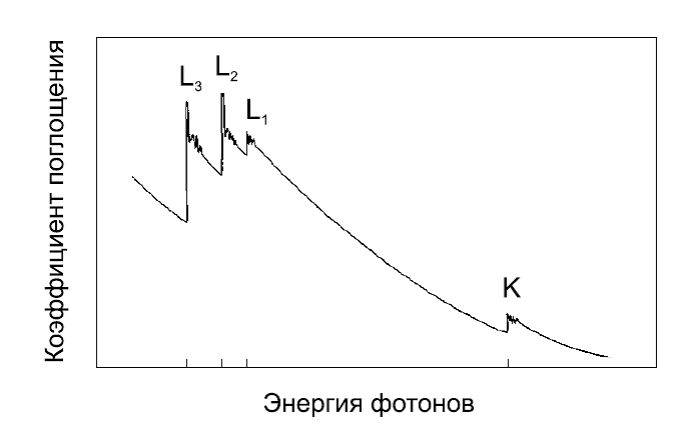
\includegraphics [scale=0.47] {./Dissertation/images/nexafs.png}
  \caption{Характерная зависимость коэффициента поглощения рентгеновского излучения от
энергии фотонов [164].} 
  \label{img:nexafs}  
\end{figure}
Для слоистых систем с $sp^2$ гибридизацией метод исследования БТСРСП позволяет получить информацию не только об интегральной плотности свободных состояний, но также выделить вклад в электронную структуру $\pi$ и $\sigma$ орбиталей, а также определить их ориентацию относительно плоскости поверхности образца. Для этого используется излучение с линейной поляризацией. Спектры поглощения снимаются при разных углах падения излучения на образец, и в зависимости от угла между направлением связи и вектором поляризации изменяется вероятность возбуждения электронов в состояния различной направленности. Так, если $\sigma$ связи находятся в плоскости поверхности образца, а $\pi$ перпендикулярны ей, то интенсивность переходов в $\sigma^*$ состояния будет максимальна при падении излучения по нормали к образцу, поскольку в этом случае вектор поляризации будет направлен вдоль $\sigma$ связей. Вероятность перехода в $\pi^*$ состояния при этом будет нулевой. Ситуация поменяется на противоположную, если направить линейно поляризованное излучение по касательной к поверхности образца.
Для изучения БТСРСП необходим источник излучения, позволяющий варьировать энергию фотонов с достаточно малым шагом, поскольку важная информация может содержаться в незначительном изменении энергетическо го положения (< 0.2 эВ), относительной интенсивности или расщеплении пиков тонкой структуры. Эксперименты по исследованию БТС проводятся с использованием синхротронного излучения. Каналы вывода синхротронного
излучения из накопителя в экспериментальную камеру содержат множество оптических элементов, например, фокусирующие зеркала и решётки монохроматора.
\section{ Экспериментальная станция}
 \begin{figure}[ht] 
  \center
  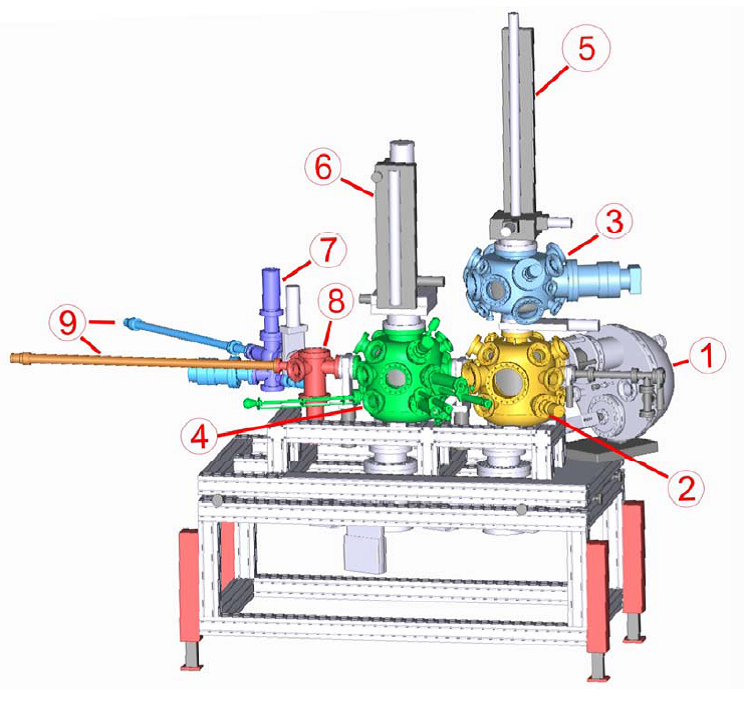
\includegraphics [scale=0.47] {./Dissertation/images/station.png}
  \caption{Изображение станции RGBL на синхротроне BESSY II: 1 - полусферический анализатор, 2 - аналитическая камера, 3, 4 - препарационные камеры, 5, 6 - стойки вертикального перемещения образцов, 7 - загрузочная камера, 8 - камера замены образцов, 9 - система горизонтального перемещения образцов.} 
  \label{img:bessy}  
\end{figure}
Результаты экспериментов, описанные в настоящей работе, получены в Российско-Германской лаборатории на синхротроне BESSY II. Схема экспериментальной станции показана на Рис. \ref{img:bessy}. Две основных части станции - препарационная и аналитическая камеры. В препарационной камере проводился отжиг образца, контроль его струкутуры методом ДМЭ и напыление железа. В аналитической камере проводились измерения спектров XPS и NEXAFS. Помимо этого на станции есть камеры загрузки и замены образцов, а также система их перемещения.

Спектры фотоэлектронной спектроскопии были получены с одного из образцов позже на станции Нанофэс синхротрона Курчатовского института.

